%!TEX root=masterproef.tex

\chapter{Implementatie}
\label{chapter:implementatie}

Voor deze thesis werd een prototype ge\"implementeerd van de generator. Hierbij
werd FOO-lang gedefinieerd tot op het niveau dat het mogelijk was om twee
realistische voorbeelden te beschrijven. Ook de generator werd uitgewerkt tot
het niveau dat het mogelijk was om de twee voorbeelden te genereren. Zowel de
voorbeelden als de implementatie van de taal en generator zijn zo uitgewerkt
dat ze als realistische referentie kunnen dienen en dat de resultaten het
potentieel waarborgen.

Het hoofdstuk wordt ingeleid met een korte sectie, \ref{section:devel-python},
over Python, de programmeertaal die werd gekozen voor de implementatie van het
prototype.

Daarna wordt FOO-lang in meer detail bekeken in sectie
\ref{section:devel-foo-lang}. Aan de hand van voorbeelden en de grammatica
introduceren we de taal, de mogelijkheden die ze biedt alsook de beperkingen
die ze introduceert. Een elementair voorbeeld wordt vervolgens als rode draad
doorheen het hoofdstuk gebruikt om de volledige generatie van FOO-lang
beschrijving tot C programmacode te illustreren aan de hand van een effectief
voorbeeld.

Sectie \ref{section:devel-codegen} belicht de generator met in hoofdzaak de
tweeledige taxonomie van het SM en het CM. De verschillende transformaties die
uitgevoerd worden op beide modellen worden kort samengevat en het onderliggende
implementatie van het \emph{visitor} patroon \citep{gamma1994design} wordt
toegelicht.

De generator wordt vergezeld van gemeenschappelijke basisfunctionaliteit in de
vorm een softwarebibliotheek, genaamd FOO-lib. Sectie
\ref{section:devel-foo-lib} overloopt kort de verschillende modules en kadert
het geheel in de context van de generator en de taal.

\section{Python}
\label{section:devel-python}

Als programmeertaal voor het prototype werd geopteerd voor Python. Python is
een ge\"interpreteerde taal met dynamische typering die verschillende
programmeerparadigma ondersteunt: imperatief, object-geori\"enteerd en
functioneel. Dit maakt het een zeer veelzijdige taal die veel mogelijkheden
biedt.

Python is ook volledig open in zijn structuur. Alles is toegankelijk en niets
wordt verborgen. Dit laat toe om elk aspect van een gegevensstructuur of object
te manipuleren. Dit kan heel handig zijn, maar kan ook leiden tot onverwachte
neveneffecten.

Alle functionaliteit, klassen of gewone functies, worden verzameld in een
\emph{module} en andere modules kunnen vervolgens deze functionaliteit
importeren. Door de volledige transparantie en dankzij ver doorgedreven
mogelijkheden tot introspectie, kan de implementatie van een module dynamisch
aangepast worden. Dit werd o.a. uitvoerig toegepast voor het implementeren van
het \emph{visitor} patroon, verder besproken in sectie
\ref{subsubsection:devel-visitor-pattern}.

Ofschoon mijn ervaring met Python beperkt was, is Python zeker geen slechte
keuze voor de implementatie van deze software. Zo beschikt de taal over een
zeer rijke verzameling van kant-en-klare modules, die toelaten om enkele
basistaken snel te implementeren. De flexibiliteit en de mix van zowel
imperatief als object-geori\"enteerd als functioneel programmeren liet
meermaals toe om bepaalde zaken op creatieve manier te implementeren.

Het feit dat in essentie een nieuwe taal was, bracht ook een bijkomende
leercurve met zich mee. Ook zorgde voortschrijdend inzicht voor stapsgewijze
verbeteringen aan bepaalde constructies, die echter soms door tijdbeperkingen
niet voor alle overige code konden bijgewerkt worden.

\section{FOO-lang}
\label{section:devel-foo-lang}

Maar de echte belangrijke taal in dit geval is niet Python, maar FOO-lang.
Codevoorbeeld \ref{lst:hello.foo} toont de implementatie van een elementair voorbeeld
in FOO-lang. Aan de hand van dit voorbeeld introduceren we nu de typische
bouwstenen van FOO-lang en doorlopen we het hele generatieproces.

\inputminted[linenos,frame=lines,framesep=2mm,fontsize=\footnotesize]{js}{../src/foo-lang/examples/hello.foo}
\vspace{-5mm}
\captionof{listing}{Elementair voorbeeld in FOO-lang: \ttt{hello.foo}
  \label{lst:hello.foo}}
\vspace{3mm}

De code start op regel 6 met de declaratie van een \emph{module}. Een module is
een op zich staand geheel en zou bv. een detectiealgoritme kunnen zijn. Alles
wat volgt op de declaratie van de module, maakt er deel van uit.

Op regel 8 introduceren we een \emph{const}ante, \ttt{interval} en stellen die
gelijk aan \ttt{1000}. Hier zien we een eerste voorbeeld van het ontbreken van
expliciete typering in FOO-lang. Dankzij type deductie zal in dit geval het
type van \ttt{interval} overeenkomen met een \emph{IntegerType}, omdat de
waarde \ttt{1000} gevormd is als een integer getal.

Ofschoon FOO-lang ge\"introduceerd wordt als DSL voor inbraakdetectie in DSN,
specificeert het zijn domein als dat van \emph{sensorknopen} of \emph{nodes}.
Algoritmes met betrekking tot inbraakdetectie in DSN, hebben \'e\'en belangrijk
gemeenschappelijke entiteit en dat zijn de sensorknopen. Deze communiceren met
elkaar en op basis van die communicatie zijn zowat alle algoritmes opgebouwd.

Het concept van een knoop of \emph{node} wordt beheert door het raamwerk dat
opgebouwd wordt door de generator. De algoritmes krijgen toegang tot deze
knopen via een aantal functionele constructies. Maar ze kunnen de
basisdefinitie van een knoop in het domein uitbreiden met hun eigen
eigenschappen. Dit gebeurt bv. op regel 10, waar (de knoop van) het domein
uitgebreid wordt met een eigenschap \ttt{sequence}. Deze eigenschap wordt
expliciet getypeerd met het \emph{byte} type en krijgt als initi\"ele waarde
\ttt{0}.

FOO-lang is een \emph{functie}-geori\"enteerde taal die tracht om de functies
in de verschillende modules, zo te organiseren dat de uitvoering ervan de \mcu
of de draadloze radio zo min mogelijk belast. Op regel 14 wordt een functie
gedefinieerd, genaamd \ttt{step}. Ze accepteert \'e\'en parameter, genaamd
\ttt{node}. We merken opnieuw op dat deze parameter niet getypeerd is.

De inhoud van de functie bestaat uit programmeerconstructies die niet ongewoon
zullen overkomen en feitelijk bijna gewone C code zou kunnen zijn. Een
conditie, een eigenschap, een waardeverhoging,\dots We zien hier onze eerder
toegevoegde eigenschap, \ttt{sequence}, terug opduiken.

Regel 20 brengt alle voorgaande definities nu samen in een
\emph{uitvoeringsstrategie}. FOO-lang tracht doormiddel van zijn syntax ook te
lezen als een natuurlijk taal. Indien we regel 20 gewoon lezen, zou dit iets
kunnen opleveren als ``\emph{At every (passing of) interval with nodes do (the
function named) step.}''. En dat is exact wat deze regel definieert.

In deze ene regel zien we de klassieke lus over alle gekende knopen die in
zowat alle algoritmen wel in \'e\'en of andere vorm terugkomt, echter nu is de
lus geabstraheerd tot zijn functionele betekenis.

\subsection{Syntax en grammatica}
\label{subsection:devel-foo-lang-grammar}

Het voorgaande voorbeeld gebruikt slechts een kleine subset van de volledige
mogelijkheden van FOO-lang. De volledige grammatica van FOO-lang, zoals
gedefinieerd in het kader van dit prototype, is opgenomen in appendix
\ref{appendix:foo-lang-grammar}. Deze appendix bevat de \emph{Extended
Backus-Naur Form} (EBNF) die de taal eenduidig bepaalt, alsook een visualisatie
van de verschillende regels.

We bespreken hier kort enkele constructies die nog niet eerder voorkwamen.

\subsubsection{Importeren van functionaliteit}

Het is mogelijk om externe functies te importeren. Dit gebeurt aan de hand van
de constructie \ttt{from ... import ... }. Hiermee wordt een functie
ge\"importeerd vanuit een module. Zo'n module kan een andere FOO-lang module
zijn, of een extern gedefinieerde functie uit een softwarebibliotheek. In
\ref{section:devel-foo-lib} introduceren we de FOO-lib, de standaard
softwarebibliotheek die de code generatie vervolledigd. Hieruit worden typisch
functies geraadpleegd in de meeste beschrijvingen.

\subsubsection{Reageren op gebeurtenissen}

Naast het herhaaldelijk uitvoeren van een functie is het ook mogelijk om een
functie te koppelen aan een gebeurtenis in de context van het domein en de
knopen. In plaats van de \ttt{with ... do} constructie is het ook mogelijk om
een voor of na (\ttt{before} en \ttt{after}) de uitvoering van een functie
binnen het kader van het domein, een functie uit te voeren. Codevoorbeeld
\ref{lst:foo-event_handler} geeft een eenvoudig voorbeeld waarbij we ontvangen
berichten tellen als deze aan ons geadresseerd waren.

\begin{listing}[ht]
  \begin{minted}[linenos,frame=lines,framesep=2mm,fontsize=\footnotesize]{javascript}
after nodes receive do function(me, sender, from, hop, to, payload) {
  if(to == me) {
    me.msg_count++
  }
}
  \end{minted}
  \vspace{-5mm}
  \caption{Voorbeeld van het reageren op een gebeurtenis}
  \label{lst:foo-event_handler}
\end{listing}

In dit voorbeeld merken we ook op dat functies anoniem kunnen gedefinieerd
worden en niet eerst met een naam gedefinieerd worden.

\subsubsection{Verschillende situaties afhandelen}

Het \ttt{case statement} laat toe om eenzelfde expressie te evalueren in
verschillende situaties. Typisch gebruik voor deze constructie is het
analyseren van ontvangen gegevens. Codevoorbeeld \ref{lst:foo-case} illustreert dit.

\begin{listing}[ht]
  \begin{minted}[linenos,frame=lines,framesep=2mm,fontsize=\footnotesize]{javascript}
after nodes receive do function(me, sender, from, hop, to, payload) {
  case payload {
    contains([#marker1, value]) {
      sender.msg_sent1++
    }
    contains([#marker2, value]) {
      sender.msg_sent2++
    }
    else {
      sender.msg_other++
    }
  }
}
  \end{minted}
  \vspace{-5mm}
  \caption{Voorbeeld van het afhandelen van verschillende situaties}
  \label{lst:foo-case}
\end{listing}

In dit voorbeeld wordt de ontvangen berichten geanalyseerd en gecatalogeerd op
basis van de inhoud. Als in een berichte \ttt{\#marker1} wordt gevonden wordt
\ttt{msg\_sent1} verhoogd, in het geval van \ttt{\#marker2}, \ttt{msg\_sent2}
en anders \ttt{msg\_other}.

Deze constructie is in feite een mooiere syntax voor een overeenkomstige
constructie op basis van \ttt{if statements}, zoals weergegeven in listing
\ref{lst:foo-case-if}.

\begin{listing}[ht]
  \begin{minted}[linenos,frame=lines,framesep=2mm,fontsize=\footnotesize]{javascript}
after nodes receive do function(me, sender, from, hop, to, payload) {
  if payload.contains([#marker1, value]) {
    sender.msg_sent1++
  } else if payload.contains([#marker2, value]) {
    sender.msg_sent2++
  } else {
    sender.msg_other++
  }
}
  \end{minted}
  \vspace{-5mm}
  \caption{Alternatieve constructie voor verschillende situaties}
  \label{lst:foo-case-if}
\end{listing}

Dit voorbeeld introduceert tevens nog drie andere belangrijke constructies: het
\emph{atom}, lijsten en patroon koppeling.

\subsubsection{Atomen}

\emph{Atomen} werden ontleed aan Erlang. Ze stellen een uniek herkenbare
entiteit voor. Het is aan de generator met hulp van het platform en/of domein
en/of doeltaal om hiervoor een geschikte voorstelling te vinden.

In het geval van dit prototype werden twee bytes voorzien om een unieke
identificatie te maken van delen in berichten. De generator kan hier
verschillende strategie\"en volgen en beslissen op basis van de verschillende
\emph{atoms} die hij tegenkomt.

\subsubsection{Lijsten}

Lijsten worden voor verschillende doeleinden gebruikt. Ze worden syntactisch
gespecificeerd door middel van vierkante haken. Zo worden ze meestal al een
letterlijke voorstelling van de lijst opgenomen. In het voorbeeld in listing
\ref{lst:foo-case} is de \ttt{payload} parameter zo'n lijst. Ook het argument
van de \ttt{contains} methode die toegepast wordt op \ttt{payload} is een
lijst. De parameter verwacht echter niet echt een lijst, maar een patroon. In
dit geval is de lijst een deel van het patroon.

\subsubsection{Patroon koppeling}

Door middel van patronen kan er een kopping gemaakt worden tussen gegevens. In
het voorbeeld in codevoorbeeld \ref{lst:foo-case} accepteert de \ttt{contains}
methode op een \emph{lijst} een patroon. Dit patroon is een lijst en bestaat
uit variabele en niet-variabele elementen. De \ttt{contains} methode zal
trachten de niet-variabele elementen herkennen in de lijst en vervolgens bij
een succesvolle herkenning een kopping te maken tussen de variabele elementen
en de waarden in de oorspronkelijke lijst.

\subsubsection{Complexe types}

In codevoorbeeld \ref{lst:hello.foo} zagen we reeds kort een voorbeeld van typering.
De \ttt{sequence} eigenschap werd getypeerd als een \ttt{byte}. Naast
\ttt{byte} zijn er ook nog \ttt{integer}, \ttt{float}, \ttt{boolean} en
\ttt{timestamp} als standaard eenvoudige types.

Vergelijkbaar met lijsten is er ook het \emph{tuple} type. Dit zijn lijsten van
types en defini\"eren de types van de elementen van een lijst van vaste lengte.

Van alle types kan ook een veelvoud gedefinieerd worden door het toevoegen van
een \ttt{*} achter het type. Zo kunnen lijsten van een bepaald type
gedefinieerd worden. Gecombineerd met het \emph{tuple} type, ontstaat zo bv. de
mogelijkheid om lijsten van \emph{records} te defini\"eren.

In codevoorbeeld \ref{lst:foo-complex_type} wordt het \ttt{nodes} domein uitgebreid
met een \ttt{inbox} eigenschap. Deze bestaat uit meerdere \emph{tuples} die op
hun beurt bestaan uit een \ttt{timestamp} en meerdere \ttt{bytes}.

\begin{listing}[ht]
  \begin{minted}[linenos,frame=lines,framesep=2mm,fontsize=\footnotesize]{javascript}
extend nodes with {
  inbox : [timestamp, byte*]* = []
}
  \end{minted}
  \vspace{-5mm}
  \caption{Voorbeeld van een complex type}
  \label{lst:foo-complex_type}
\end{listing}

\subsubsection{Strings}

Grote afwezige in deze versie van FOO-lang zijn strings. Dit lijkt initieel
contra-intu\"itief, maar bij nader inzien zijn strings niet echt van toepassing
in het domein van inbraakdetectie in DSN. De introductie van strings in
FOO-lang zou op dit ogenblik tevens een herschrijven van de grammatica vragen.

\section{Code generator}
\label{section:devel-codegen}

Met FOO-lang zijn we nu in staat om inbraaddetectiealgoritmes te beschrijven.
Deze FOO-lang code moet vervolgens door de code generator omgezet worden in een
gewone programmeertaal. In het geval van dit prototype is dat C.

\subsection{Opbouw}

Figuur \ref{fig:devel-component-overview} geeft een overzicht van de opbouw van
de oplossing.

\begin{figure}[ht]
  \centering
  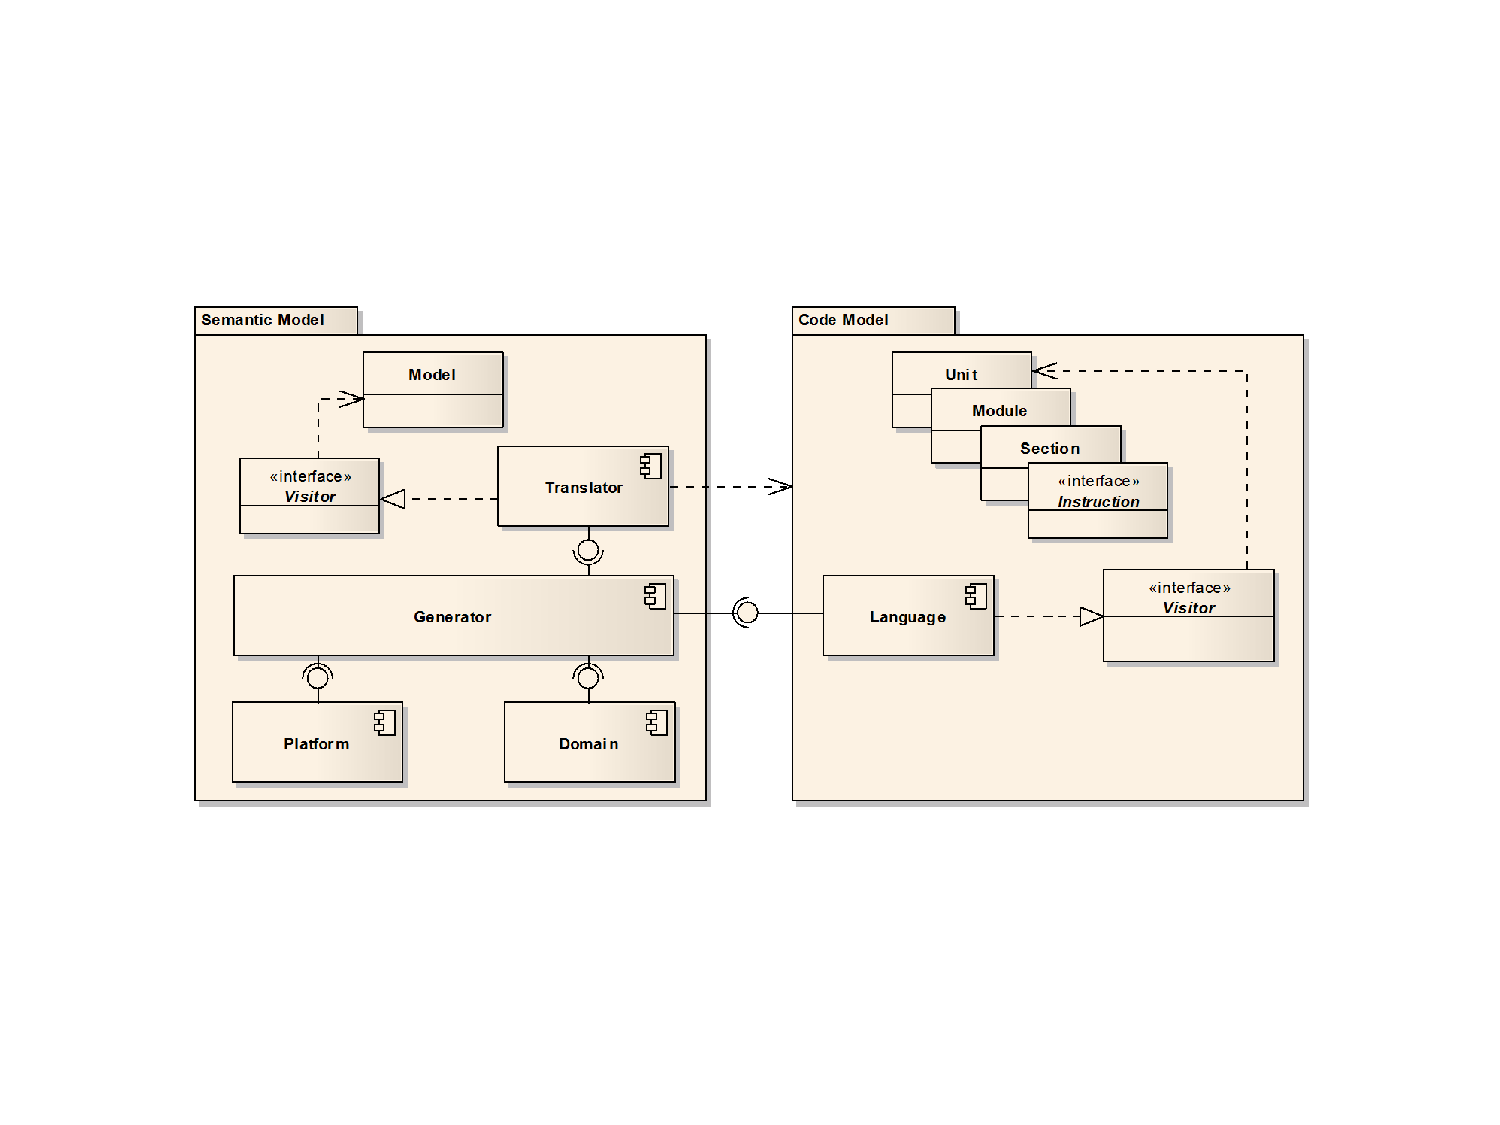
\includegraphics[width=\linewidth]{resources/component-overview.pdf}
  \caption{Overzicht van componenten en kernentiteiten}
  \label{fig:devel-component-overview}
\end{figure}

Intern bestaat de hele oplossing uit twee grote delen: het semantische en het
code gedeelte. Binnen het semantische gedeelte vinden we het SM terug. Dit
model kan benaderd worden door middel van een zgn. \emph{visitor}, een
implementatie van het \emph{visitor pattern}. Aan de hand van deze
\emph{visitor} kunnen transformaties van het model gerealiseerd worden.

Het SM is de primaire invoer voor de generator. Die kan zijn werk slechts
vervullen door middel van een compositie met \emph{platform-} en
\emph{domeininformatie}, een vertaler (Engels: \emph{Translator}) die elementen
uit het semantische gedeelte kan omzetten naar overeenkomstige elementen in het
code gedeelte en de uiteindelijk beoogde programmeertaal (Engels:
\emph{Language}).

De programmeertaal maakt deel uit van het CM. Dit is op zijn beurt opgebouwd
uit een hi\"erarchie van vier niveaus. De structuur van de beoogde code wordt
weergegeven door de compilatie \emph{unit}, de \emph{modules} en de
\emph{secties}, waarbij de unit staat voor het geheel, de modules voor
functioneel samenhangende delen en de secties zorgen voor een fysieke opdeling
in bv. bestanden. De juiste realisatie van deze hi\"erarchie wordt overgelaten
aan de implementatie van de taal die hier betekenis kan aan geven.

Op het laagste niveau van het CM vinden we de \emph{instructies}. Deze kunnen
gebruikt worden om de effectieve code voor te stellen. Er bestaat in het CM per
definitie een overeenkomstige instructie voor elk element uit het SM. Aangezien
het SM functioneel rijker is dan de meeste programmeertalen, zal na constructie
van het initi\"ele CM, door middel van transformaties, alternatieven
ge\"implementeerd moeten worden binnen de mogelijkheden van de uiteindelijke
programmeertaal.

\subsection{ANTLR}
\label{subsection:devel-antlr}

Maar alles begint bij het inladen van de FOO-lang bronbestanden in het SM. Dit
gebeurt door middel van een \emph{parser} die de tekstuele voorstelling
analyseert en de taal-eigen constructies er uit puurt. Het resultaat van deze
stap is de constructie van een boomstructuur die de juiste semantische
betekenis van de verschillende constructie structureel weergeeft. Zo'n
boomstructuur is een AST. Figuur \ref{fig:devel-ast} toont de AST van het
elementaire voorbeeld uit codevoorbeeld \ref{lst:hello.foo}.

\begin{figure}[ht]
  \centering
  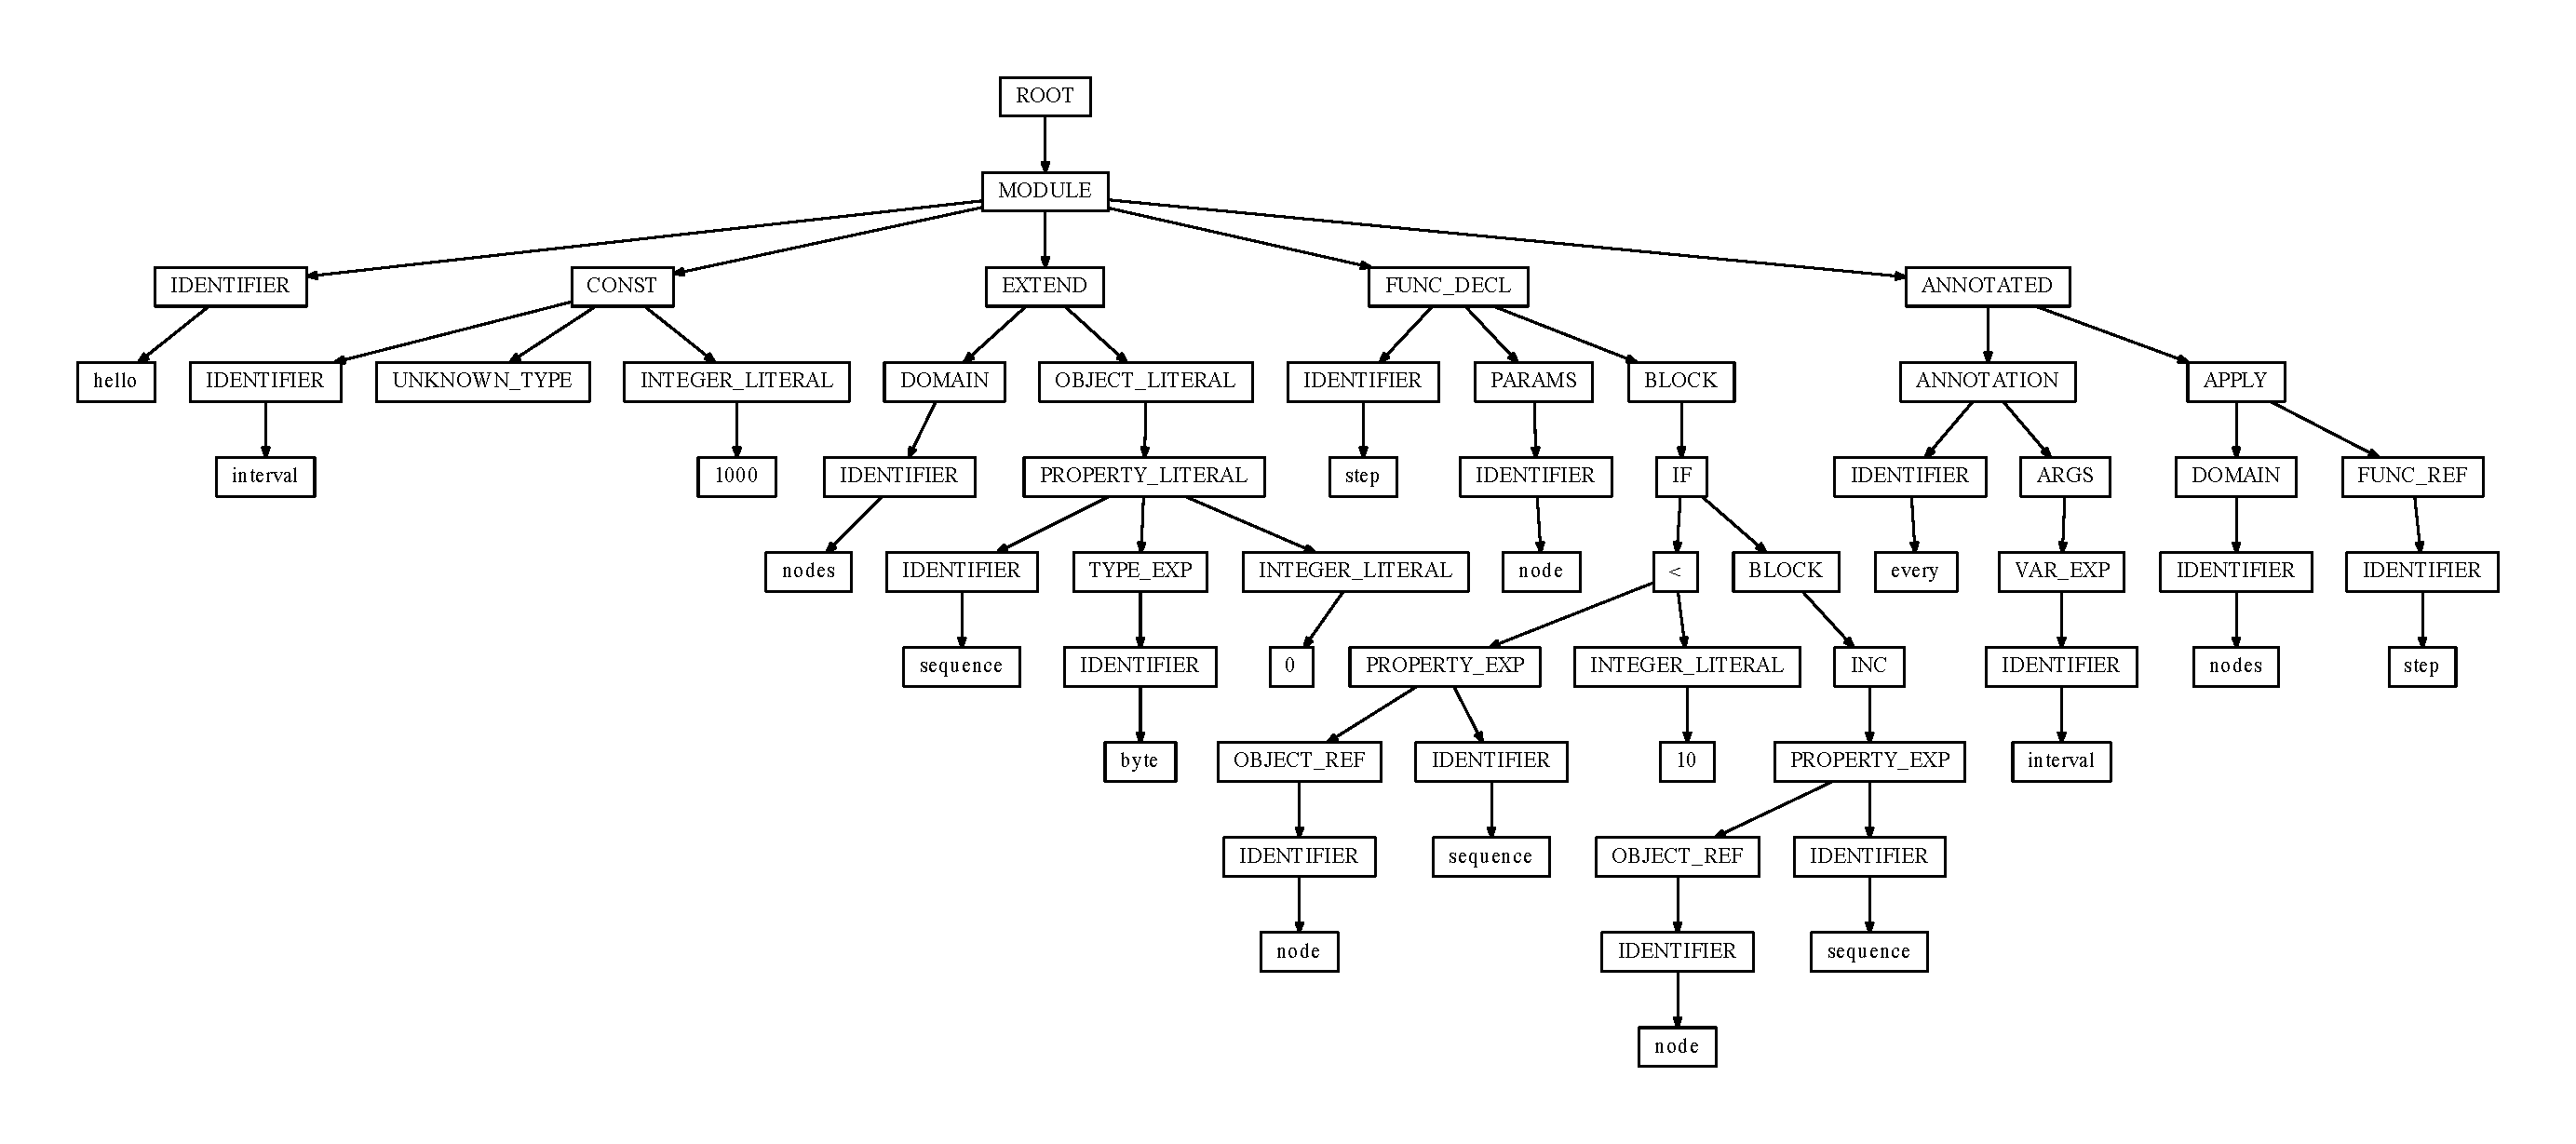
\includegraphics[width=\linewidth]{resources/hello_ast.pdf}
  \caption{De AST van het elementaire voorbeeld, \ttt{hello.foo}}
  \label{fig:devel-ast}
\end{figure}

We herkennen duidelijk de inhoud van het codevoorbeeld: op het hoogste niveau
zien we de module met een naam, de definitie van een constante, een uitbreiding
van het domein, een functie definitie en een geannoteerde applicatie van een
functie op een domein. De AST is ontdaan van alle ondersteunende syntax zoals
aanduidingen voor blokken code,\dots en bevat louter de semantische inhoud.

\subsection{Interfaces}
\label{subsection:devel-codegen-interfaces}

Voor we het SM en het CM in detail bekijken, kijken we eerst naar de interfaces
die de code generator ter beschikking stelt.

\subsubsection{foo.py}

Op het hoogste niveau biedt de generator een commandolijn interface (CLI) aan
in de vorm van een Python script: \ttt{foo.py}. Codevoorbeeld \ref{lst:foo.py-help}
toont de uitvoering van het script die een overzicht geeft van de mogelijkheden.

\begin{listing}[ht]
  \begin{minted}[linenos,frame=lines,framesep=2mm,fontsize=\footnotesize]{console}
$ source setpath.sh
$ ./foo.py --help
usage: foo.py [-h] [-v] [-c] [-i] [-g FORMAT] [-o OUTPUT] [-l LANGUAGE]
              [-p PLATFORM]
              [sources [sources ...]]

Command-line tool to interact with foo-lang and its code generation
facilities.

positional arguments:
  sources               the source files in foo-lang

optional arguments:
  -h, --help            show this help message and exit
  -v, --verbose         output info on what's happening
  -c, --check           perform model checking
  -i, --infer           perform model type inferring
  -g FORMAT, --generate FORMAT
                        output format (choices: none, ast, ast-dot, sm-dot,
                        foo, code / default: none)
  -o OUTPUT, --output OUTPUT
                        output directory (default: .)
  -l LANGUAGE, --language LANGUAGE
                        when format=code: target language (choices: c /
                        default: c)
  -p PLATFORM, --platform PLATFORM
                        when format=code: target platform (choices: moose,
                        demo / default: moose)
  \end{minted}
  \vspace{-5mm}
  \caption{Informatie over de werking van \ttt{foo.py}}
  \label{lst:foo.py-help}
\end{listing}

De CLI biedt toegang tot alle aspecten van de generator: model controle
(\ttt{check}), type deductie (\ttt{infer}), het uitvoerformaat, waar de uitvoer
moet geplaatst worden, welke taal gebruikt moet worden en voor welk platform de
generatie moet gebeuren.

De lijst van mogelijke uitvoerformaten bestaat uit: \ttt{none}, \ttt{ast},
\ttt{ast-dot}, \ttt{sm-dot}, \ttt{foo} en \ttt{code}.

Formaat \ttt{ast} toont een hierarchisch overzicht van de AST op het scherm in
tekstuele vorm, zoals weergegeven in codevoorbeeld \ref{lst:foo.py-ast}. De
uitvoer van \ttt{ast-dot} zagen we in essentie reeds eerder in figuur
\ref{fig:devel-ast}. De uitvoer is feitelijk code die als invoer kan dienen
voor GraphViz \citep{url:graphviz}, een open bron project dat zich
specialiseert in het visualiseren van graafgeori\"enteerde gegevens, zoals deze
AST met een boomstructuur. Door middel van het \ttt{dot} commando kan
vervolgens van deze code een visuele voorstelling gemaakt worden.

\begin{listing}[ht]
  \begin{minted}[linenos,frame=lines,framesep=2mm,fontsize=\footnotesize]{console}
$ source setpath.sh
$ ./foo.py -g ast examples/hello.foo 
ROOT
  MODULE
    IDENTIFIER
      hello
    CONST
      IDENTIFIER
        interval
      UNKNOWN_TYPE
      INTEGER_LITERAL
        1000
    EXTEND
...
  \end{minted}
  \vspace{-5mm}
  \caption{Tekstuele uitvoer van een AST}
  \label{lst:foo.py-ast}
\end{listing}

Overeenkomstig bestaat er ook de mogelijkheid om een visuele voorstelling te
maken van het SM, door middel van het \ttt{sm-dot} formaat. Om controles te
doen betreffende de goede verwerking van de FOO-lang broncode kan een ingelezen
set van modules ook opnieuw als FOO-code uitgevoerd worden.

Tot slot is er nog het \ttt{code} formaat, dat de generator vraagt om
effectieve code te genereren. Hierbij dienen dan ook de overige opties
eventueel ingevuld te worden: uitvoerlocatie, taal en platform.

\subsubsection{API}

Het \ttt{foo.py} Python script is slechts een CLI-verpakking rond de Python
API. Deze biedt alle functionaliteit aan in de vorm van een Python module met
een imperatieve interface. Codevoorbeeld \ref{lst:codegen-api} toont de interface
van deze module.

\begin{listing}[ht]
  \begin{minted}[linenos,frame=lines,framesep=2mm,fontsize=\footnotesize]{python}
def create_model():
  ...
  return model

def parse(string, noprint=False):
  ...
  return parser

def infer(model, silent=False):
  ...

def check(model, silent=False):
  ...

def generate(model, args):
  ...

def load(string, model=None):
  ...
  return model
  \end{minted}
  \vspace{-5mm}
  \caption{API van de code generator}
  \label{lst:codegen-api}
\end{listing}

In volgorde zien we de verschillende fasen uit het generatie proces: het
aanmaken van een (leeg) model, het parsen van de broncode, het deduceren van
onbekende types, het controleren of een model volledig in orde is en
uiteindelijk het genereren van de code. De bijkomende \ttt{load} functie
combineert de \ttt{create\_model} en \ttt{parse} functionaliteit in \'e\'en
handige functie.

De API laat toe om de generator vanuit Python aan te spreken en eventueel
verder te integreren in een uitgebreider compilatieproces, of om andere
interfaces te voorzien (visuele gebruikersinterfaces zoals bv. een
webinterface,\dots).

De API biedt toegang tot de entiteiten op het hoogste niveau, zoals de parser,
de model-entiteit uit het SM,\dots De volledige openheid van Python code laat
verder toe om dieper door te dringen en elk aspect van het bv. model te
ondervragen of zelfs te wijzigen.

Beide onderliggende modellen zijn echter volledig ondervraagbaar aan de hand
van een \emph{visitor}. Deze worden door de generator veelvuldig gebruikt,
zelfs voor kleine operaties en bieden een veel aantrekkelijkere interface om
met de modellen te werken dan het ruwweg volgen van eigenschappen en methoden
doorheen het model.

\subsection{Semantisch model}
\label{subsection:devel-semantic-model}

De AST wordt door een eerste \emph{visitor} ingeladen in het SM. Dit is in
essentie een eenvoudige vertaling van de boomstructuur naar de overeenkomstige
elementen in het SM. Het resultaat kan opnieuw gevisualiseerd worden door
middel van GraphViz, zoals weergegeven in figuur \ref{fig:hello.sm}.

\begin{figure}[ht]
  \centering
  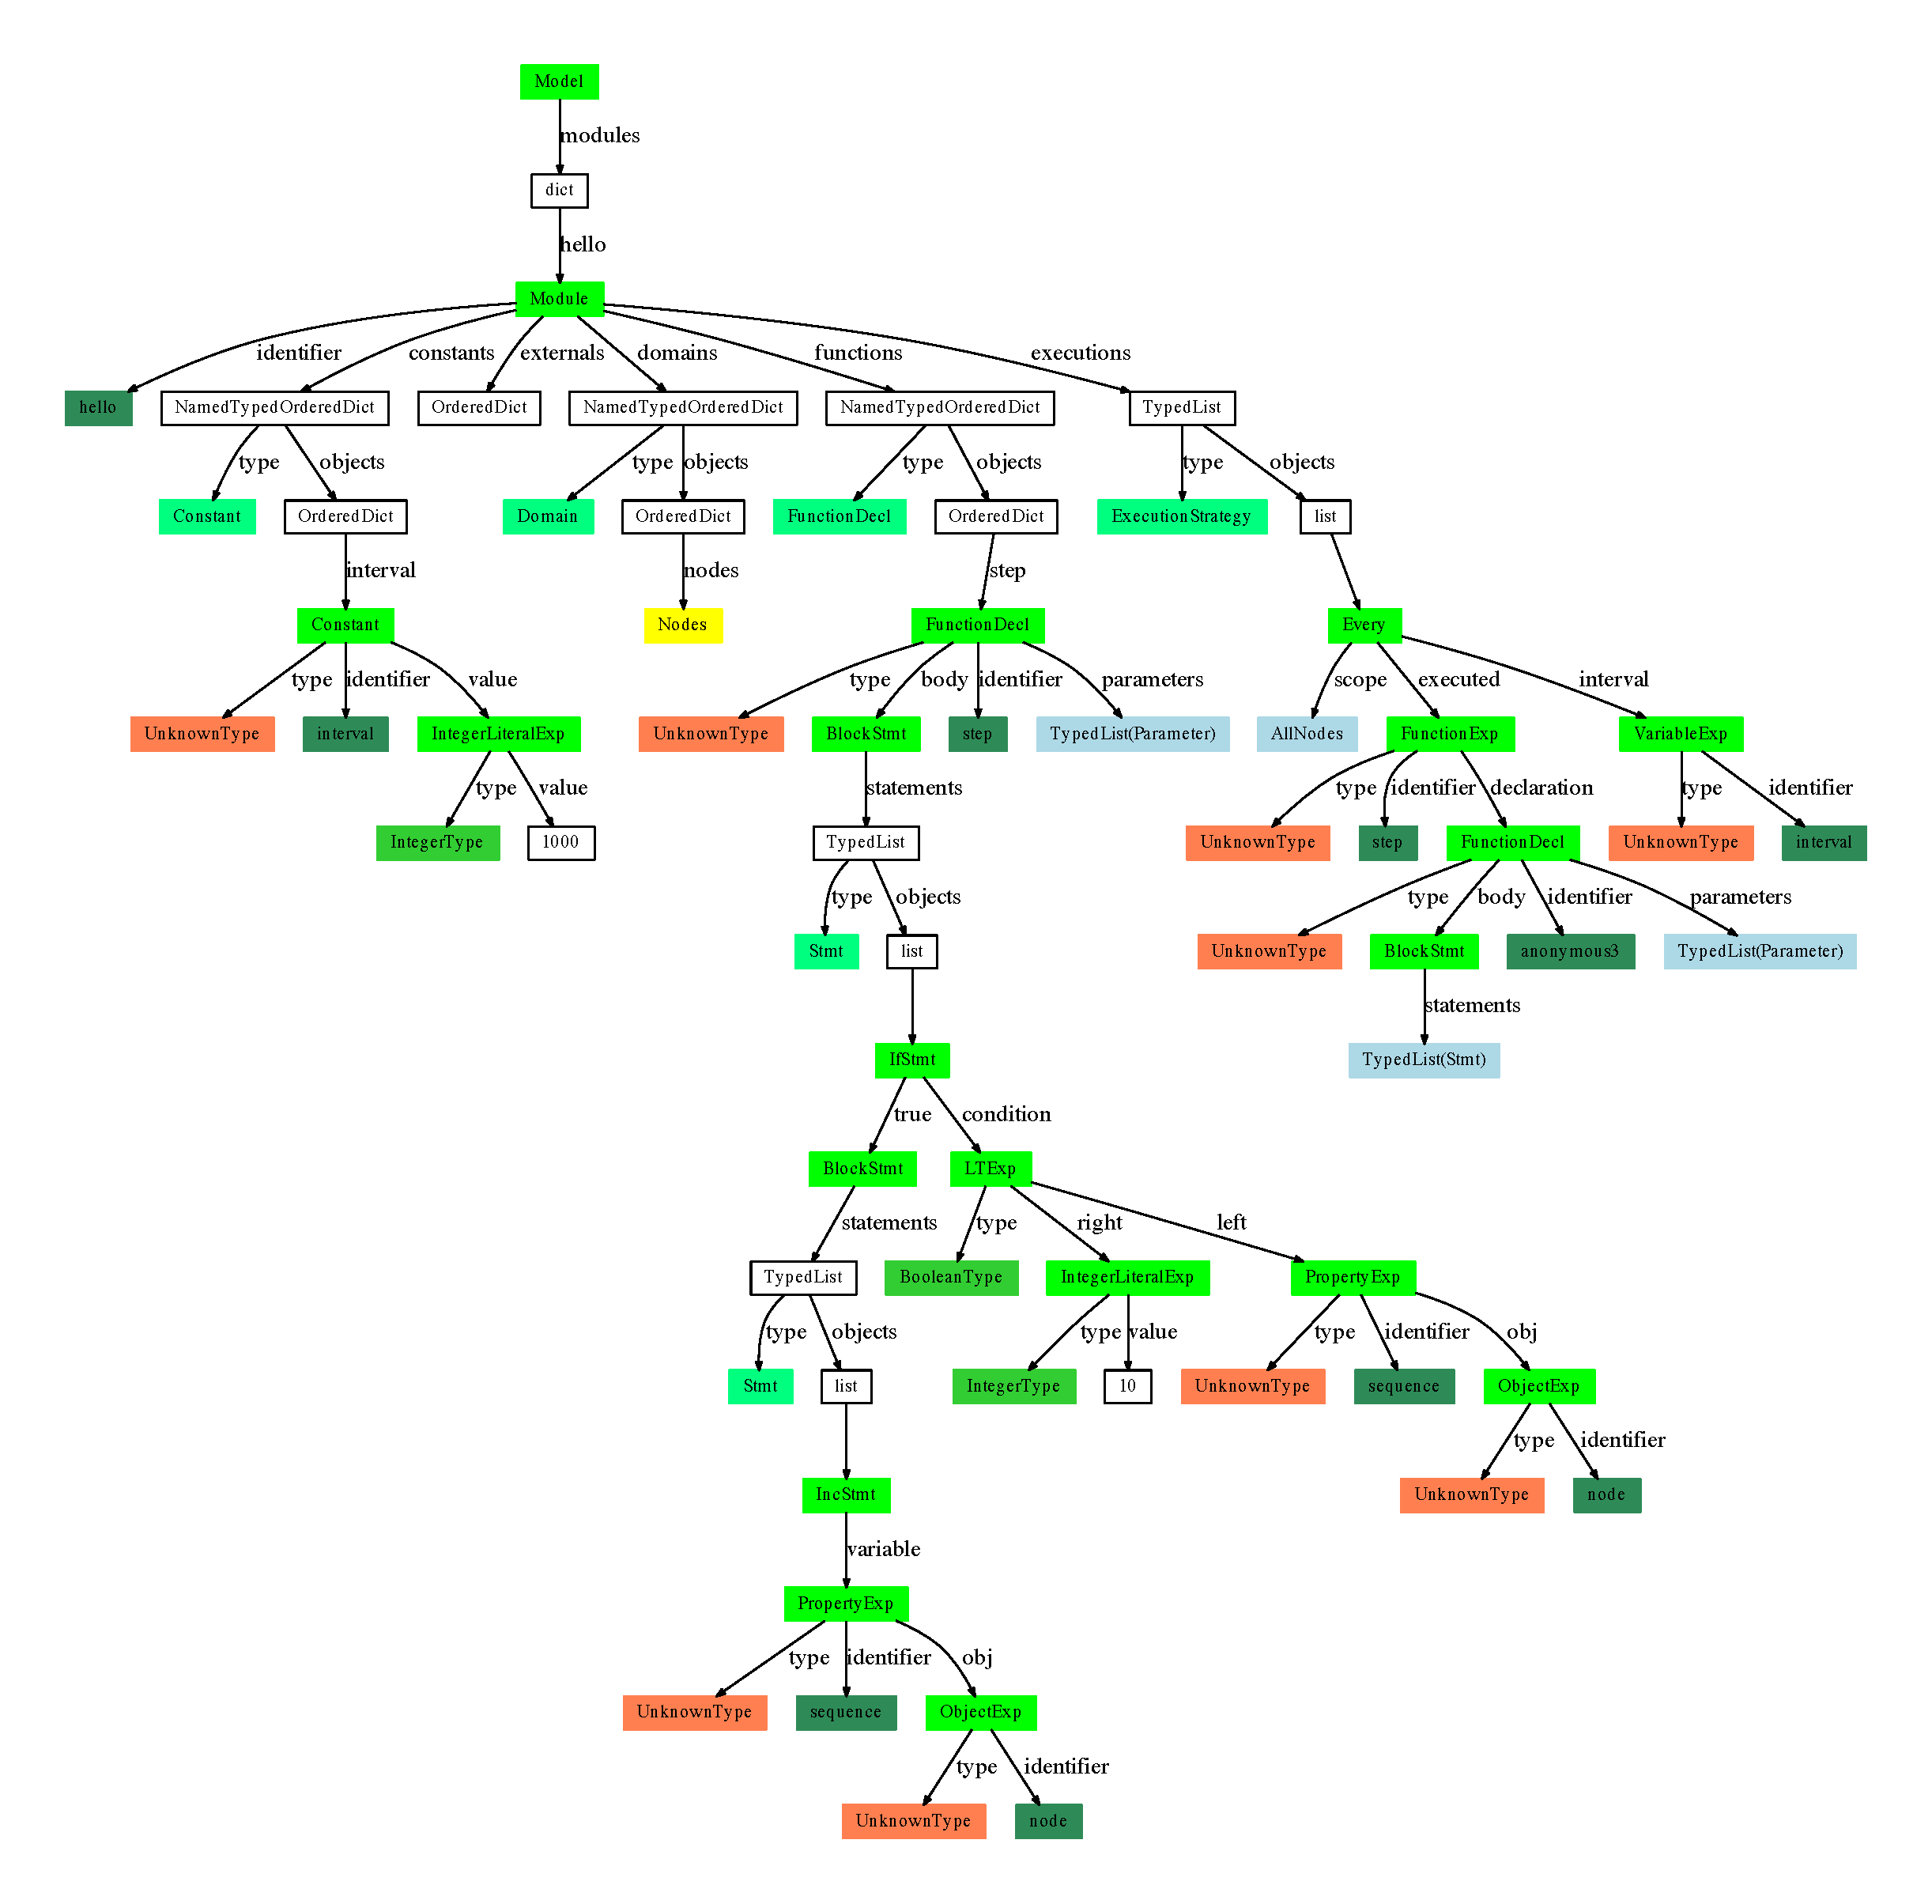
\includegraphics[width=\linewidth]{resources/hello_sm.pdf}
  \caption{Het SM van het elementaire voorbeeld, \ttt{hello.foo}}
  \label{fig:hello.sm}
\end{figure}

Bij deze visualisatie is gebruikgemaakt van een kleurencodering. Het SM kan
veel meer informatie bevatten dan de AST, zoals onder meer typering. Hierdoor
wordt de visualisatie van het SM ook een stuk groter. Dankzij de kleuren is het
makkelijker om het diagram te interpreteren.

De belangrijkste kleur is zonder meer de rode kleur. Deze geeft problemen aan
in het model. In dit geval betreft het onbekende types. Dit is in deze fase van
het generatieproces normaal aangezien typering in FOO-lang optioneel is. Deze
eerste versie van het SM bevat daarom nog niet alle types.

Een ander deel dat lijkt te ontbreken in dit diagram is de uitbreiding van het
domein. In het voorbeeld werd immers een eigenschap \ttt{sequence} toegevoegd.
Aangezien dit een uitbreiding is van het domein, zal deze terug te vinden zijn
in de eigen instantie van het domein voor deze module. In figuur
\ref{fig:hello.sm} is dit domein beperkt tot een referentie in een gele kleur.
Figuur \ref{fig:nodes.sm} toont de volledige inhoud van wat zich hierachter
verschuilt.

\begin{figure}[H]
  \centering
  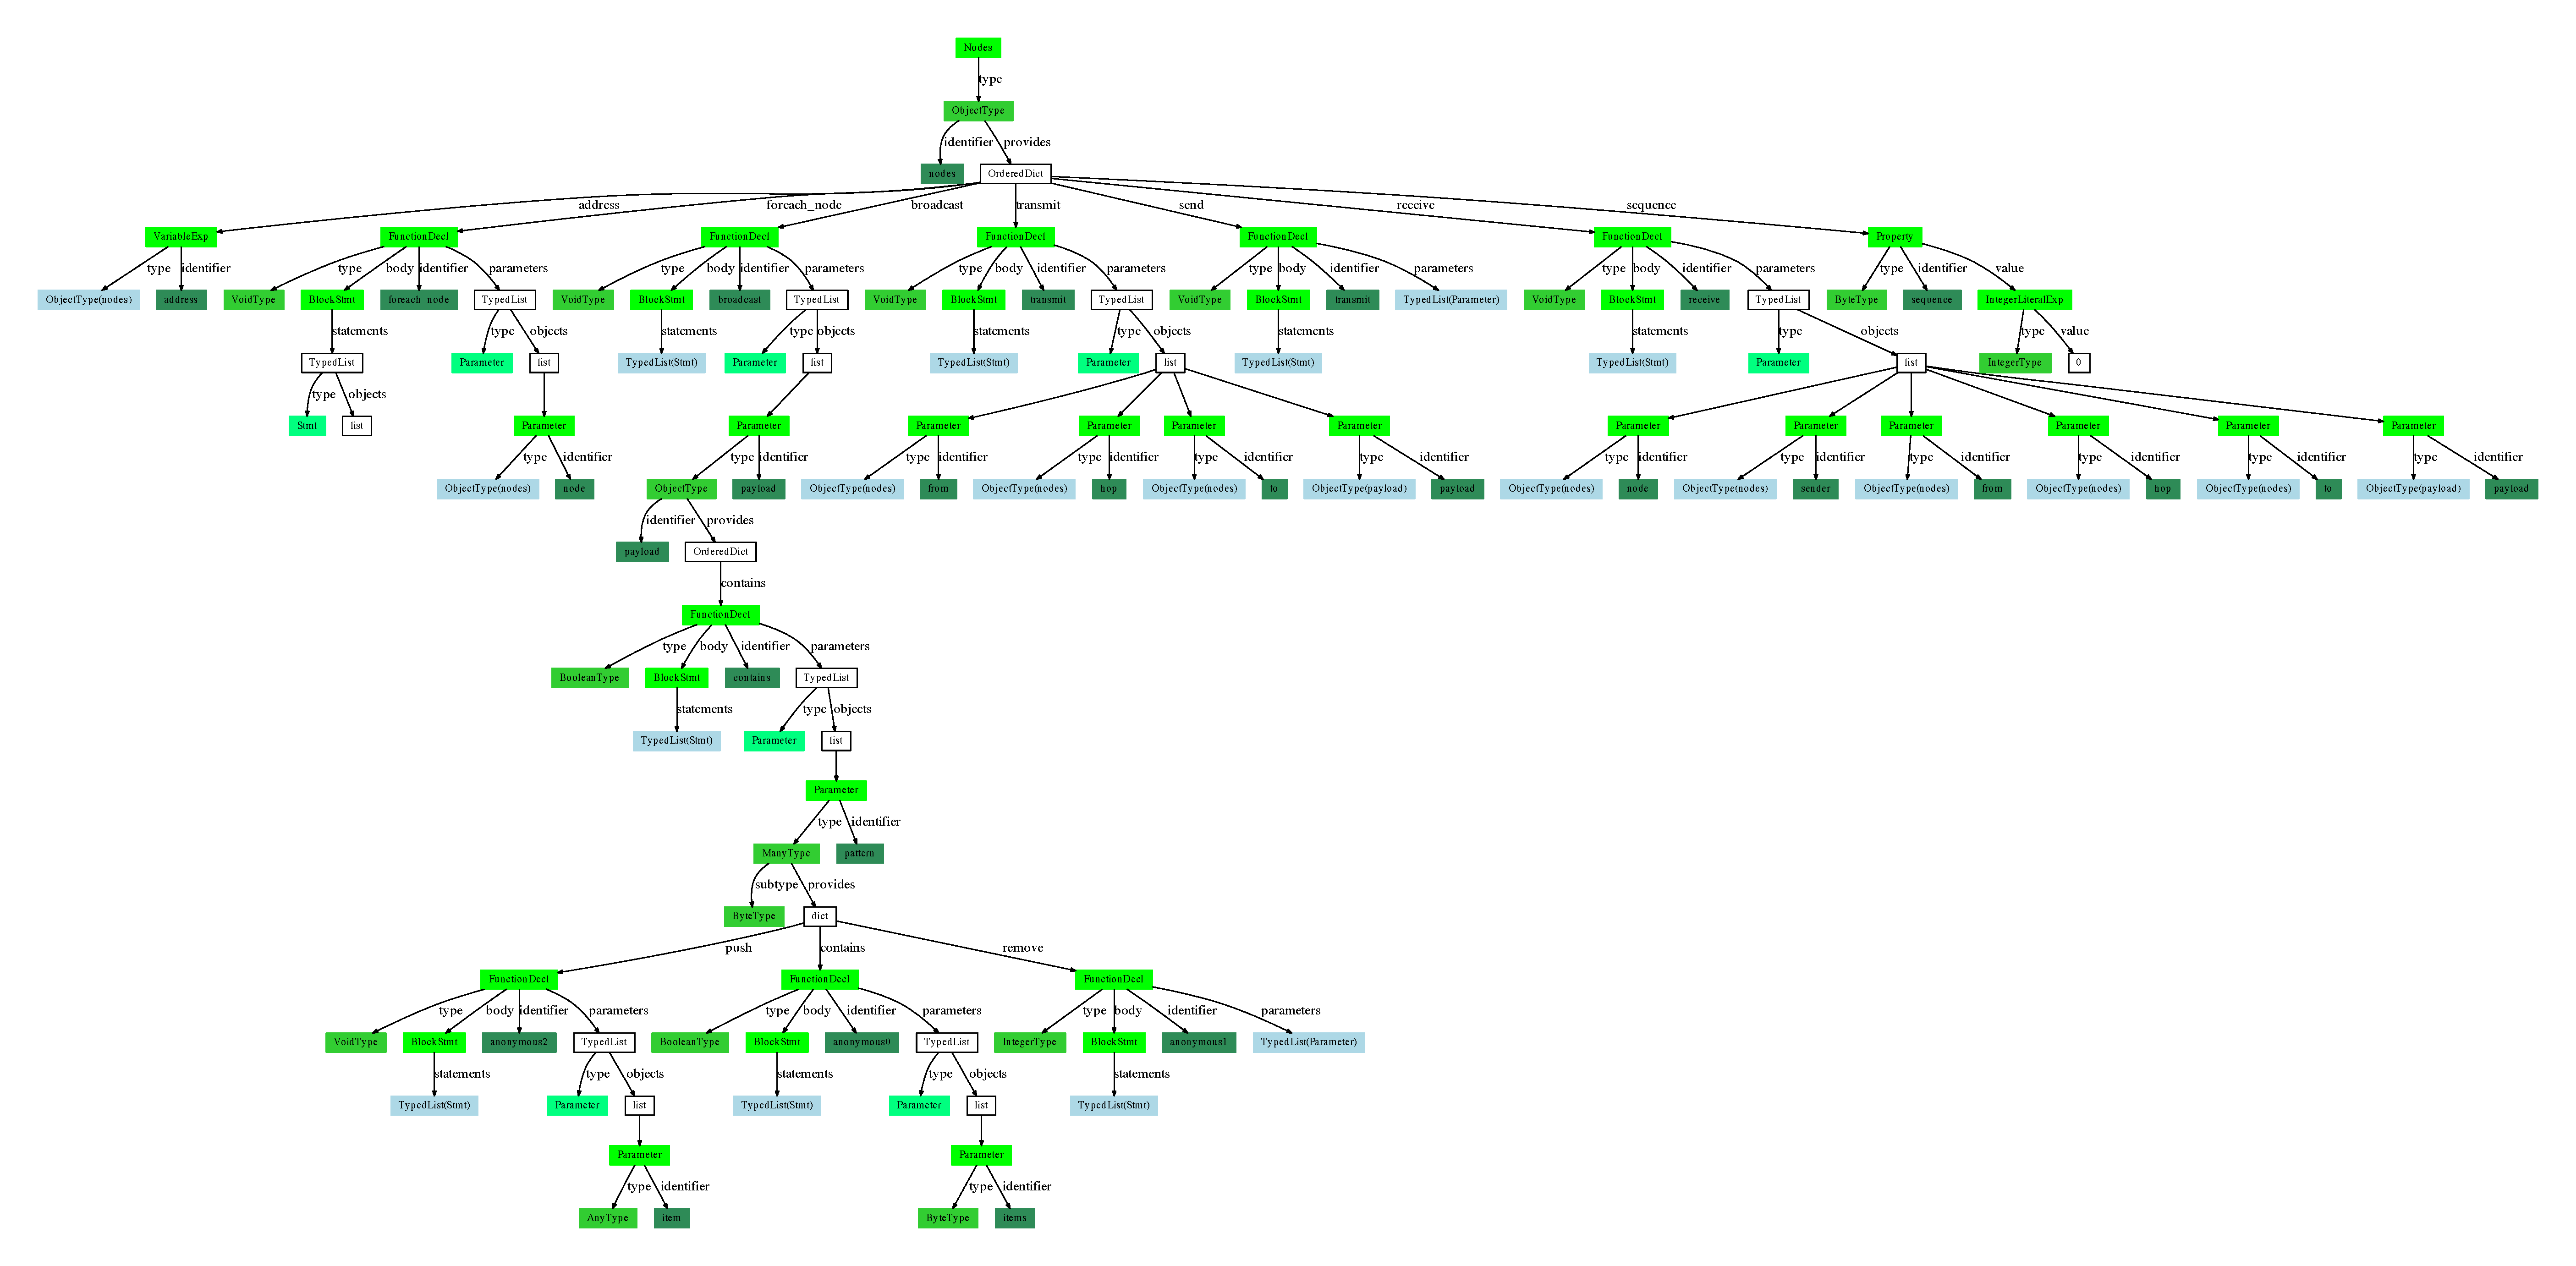
\includegraphics[angle=90,width=0.7\linewidth]{resources/nodes_sm.pdf}
  \caption{Het knopendomein in het SM voor \ttt{hello.foo} }
  \label{fig:nodes.sm}
\end{figure}

Dit is een groot stuk van het SM en behelst verschillende types en functie
declaraties die door het knopendomein ge\"introduceerd worden in het SM. Hier
zien we tevens de uitbreiding met de extra \ttt{sequence} eigenschap.

\subsubsection{Type deductie}

De volgende stap in het generatieproces bestaat erin om de nog onbekende types
te deduceren op basis van andere informatie uit het SM. Dit gebeurt aan de hand
van de \ttt{inferrer module}. Dit is een implementatie van de \emph{visitor}
voor het SM die nagaat dat alle types gekend zijn. Voor onbekende types wordt,
afhankelijk van de plaats van het type op verschillende manieren op zoek gegaan
naar een juiste typering.

De eenvoudigste methode bouwt terwijl het model doorlopen wordt een overzicht
op van gekende types die ontstaan door de declaratie van variabelen,\dots
Indien een onbekend type wordt gevonden, consulteert de \ttt{inferrer module}
dit overzicht. Indien een referentie naar een eerdere declaratie gevonden
wordt, kan het type eenvoudig gededuceerd worden.

In een aantal gevallen is de deductie niet rechtstreeks af te lezen uit
eenvoudige declaraties en moet er naar andere mogelijke combinaties gekeken
worden. Voorbeelden hiervan zijn bv. functie declaraties die gebruikt worden
als reactie op een gebeurtenis. De gebeurtenis specificeert hoe de reagerende
functie gedeclareerd is. Op basis van de omkaderende gebeurtenis moet
vervolgens het overeenkomstige prototype van de functie opgezocht en gekoppeld
worden.

Na het succesvol uitvoeren van deze type deductie zijn de voordien onbekende
types gekend en is het model volledig. Figuur \ref{fig:hello.sm-inferred} toont
hetzelfde SM als voordien, echter nu met volledig gekende typering.

\begin{figure}[ht]
  \centering
  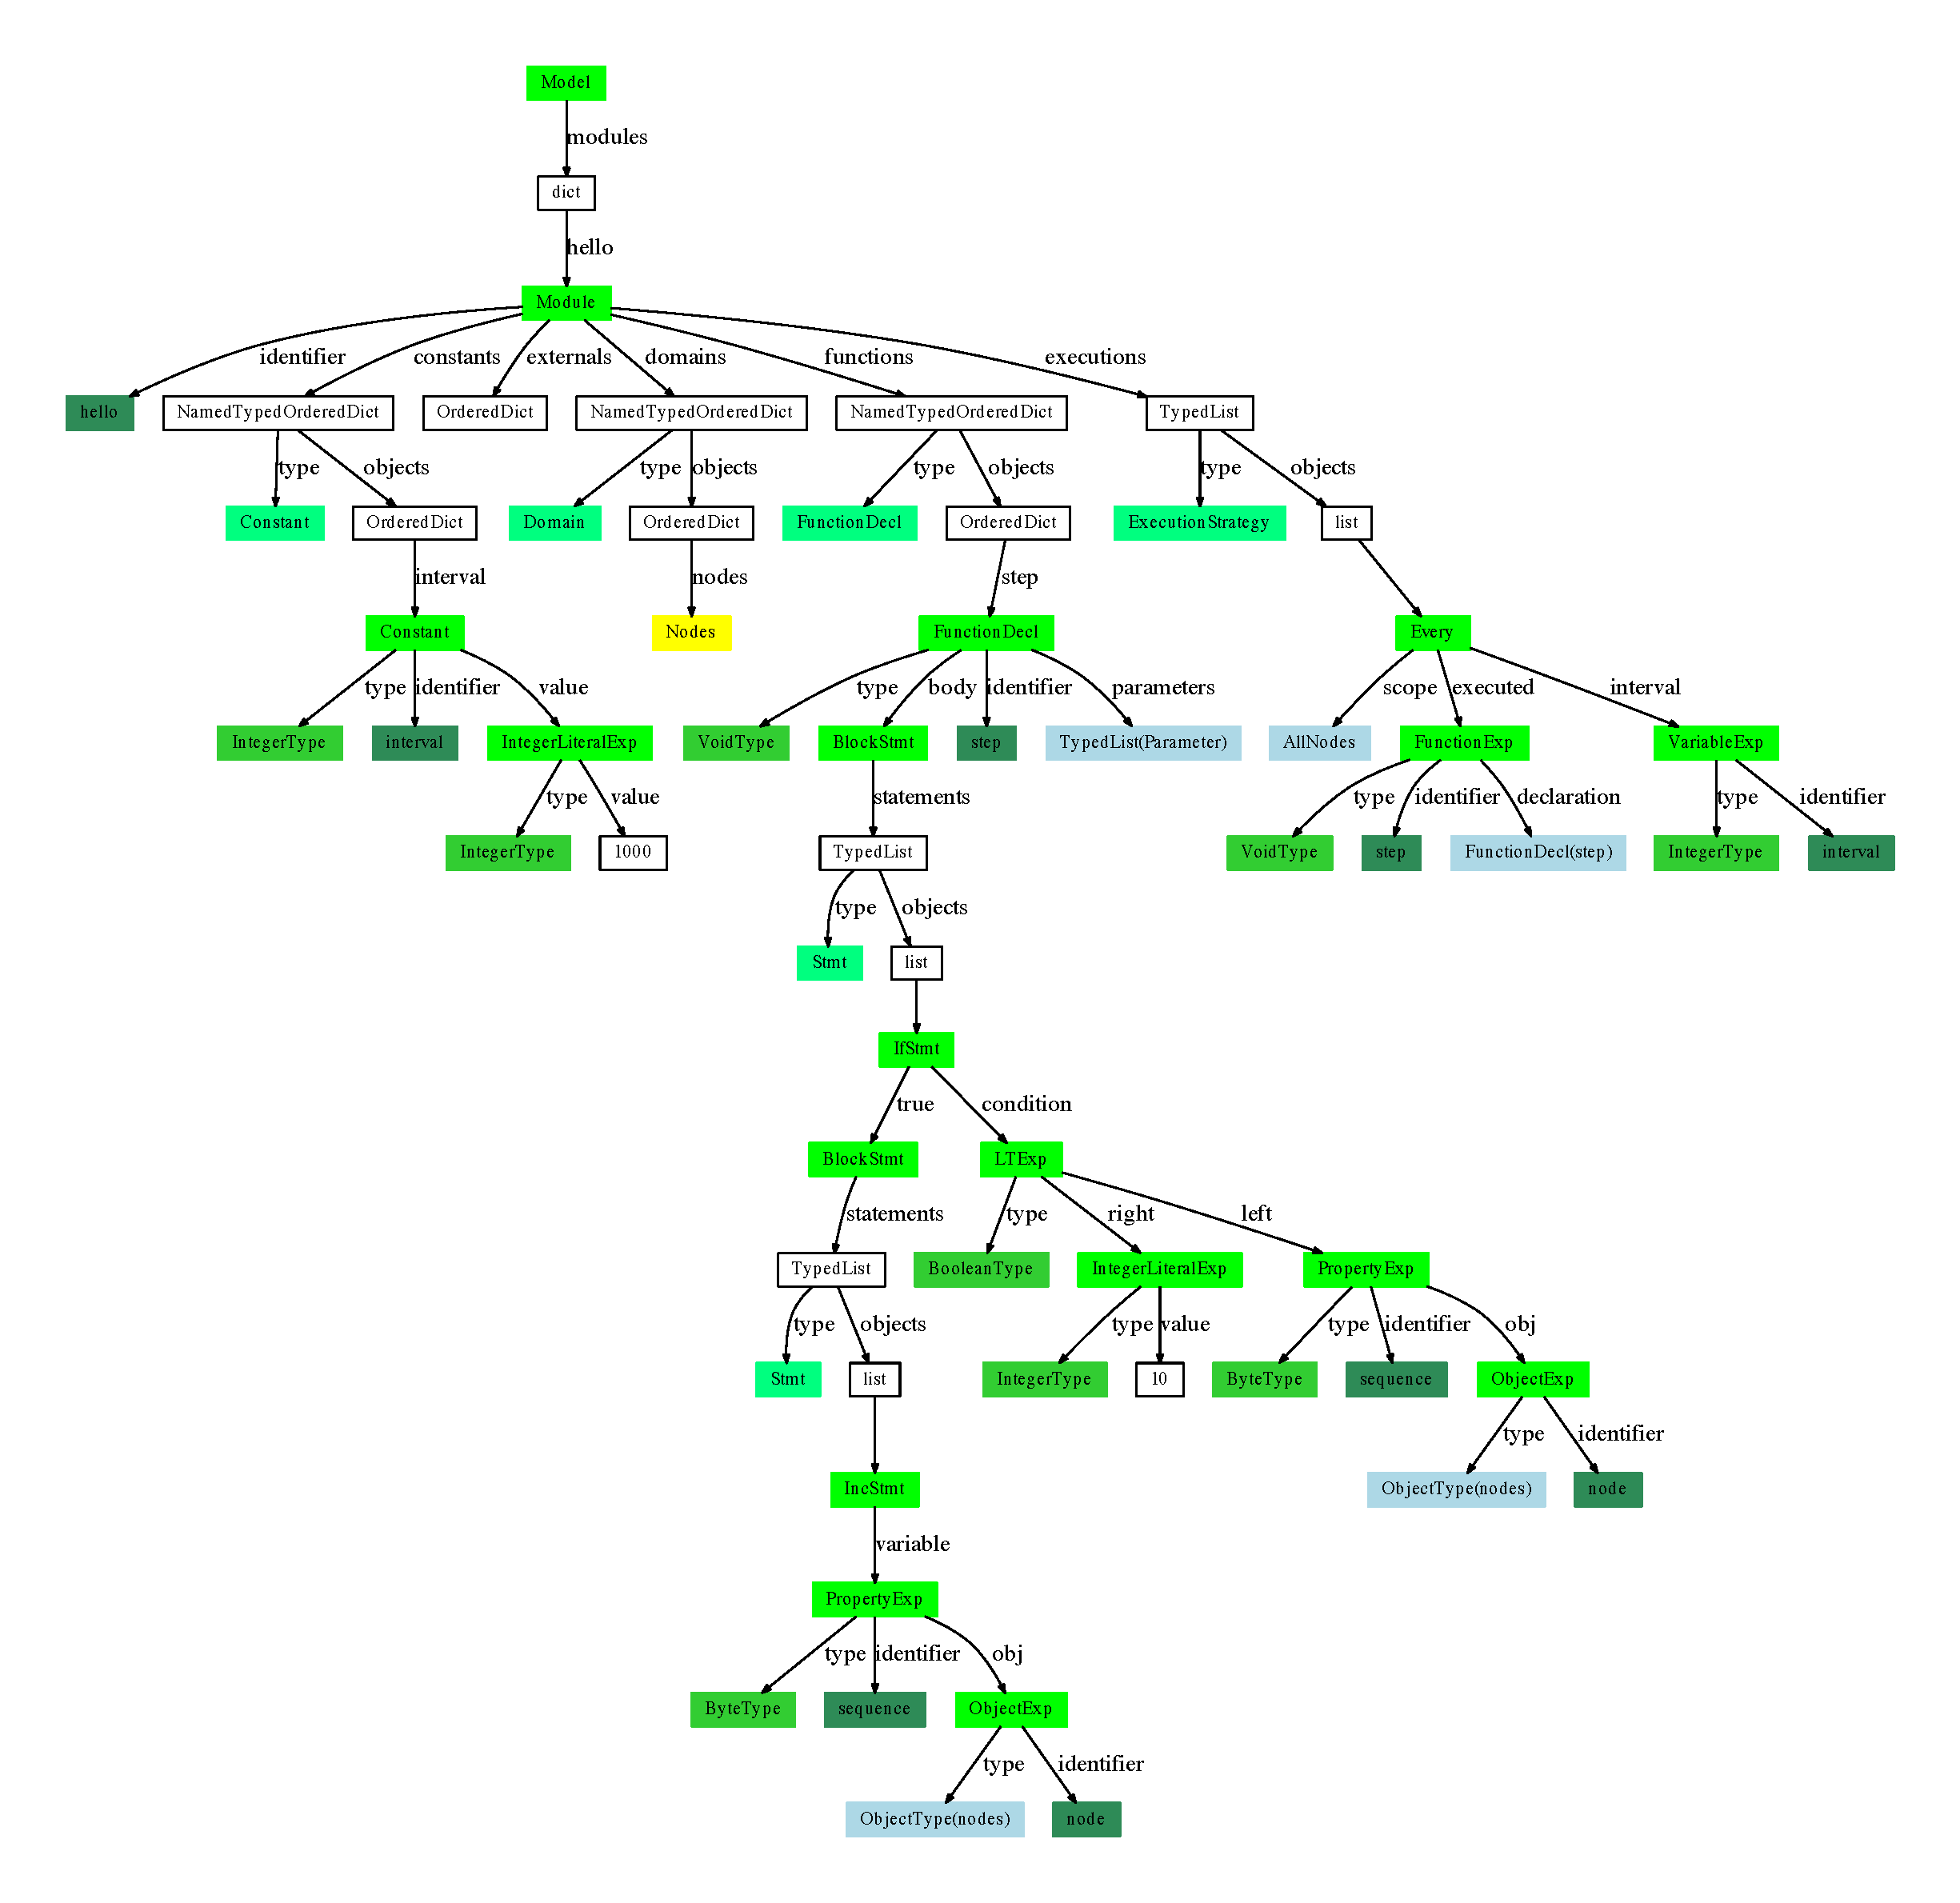
\includegraphics[width=\linewidth]{resources/hello_sm_inferred.pdf}
  \caption{Het SM van het elementaire voorbeeld, \ttt{hello.foo}, na type deductie}
  \label{fig:hello.sm-inferred}
\end{figure}

Ofschoon men verwacht dat deze fase geen structurele wijzigingen aanbrengt aan
het SM, zien we in dit geval toch dat er een vijftal elementen uit het model
verdwenen lijken te zijn. Dit is nochtans een gewoon voorbeeld van deductie. Na
het inladen van het initi\"ele model werd de (enige) uitvoeringsstrategie
gekoppeld aan een functie-expressie (\emph{FunctionExp}) genaamd, \ttt{step}.
Op dit ogenblik was er over step niets meer geweten. De declaratie van step was
wel eerder gebeurd, maar het is pas in de deductiefase dat het onbekende type
van deze functie opgezocht werd. Deel van het type is tevens de declaratie
ervan. Tijdens de deductie-fase wordt deze gekoppeld aan de eerdere declaratie,
waardoor dat in figuur \ref{fig:hello.sm-inferred} deze functiedeclaratie niet
meer volledig getoond wordt, maar nu als een referentie naar de \ttt{step}
functie opgenomen is.

\subsubsection{Model controle}

De \ttt{inferrer module} tracht alle onbekende types te deduceren. Hiermee
moeten normaal gezien de overblijvende problemen opgelost zijn. Een tweede
ondersteunende module is de \ttt{checker module} or model controle module. Deze
overloopt ook aan de hand van een \emph{visitor} het hele model en controleert
of alles in orde is.

De \ttt{checker module} is typisch nuttig bij het schrijven van FOO-lang code
en kan dienen als syntax en semantisch controle. Wanneer er bv. een schrijffout
gemaakt wordt in de naam van een variabele of functie, kan dit soms niet direct
opvallen. FOO-lang maakt bv. automatisch declaraties voor variabelen aan
wanneer zij voor het eerste gebruikt worden en nog niet eerder gedeclareerd
werden. De \ttt{checker module} kan bv. voor deze situaties waarschuwingen
geven, die kunnen helpen bij het schrijven van de FOO-lang broncode.

Ter illustratie toont codevoorbeeld \ref{lst:checker} de uitvoer van het
\ttt{hello.foo} voorbeeld. Hier is echter een \emph{fout} gemaakt in de naam
van de toegepast functie: in plaats van \ttt{step} wordt verwezen naar
\ttt{step2}.

\begin{listing}[ht]
  \begin{minted}[linenos,frame=lines,framesep=2mm,fontsize=\footnotesize]{console}
$ source setpath.sh
$ ./foo.py --check examples/hello.foo
foo-checker: failure: constant type is Unknown : interval
    stack:
      Model > Module(hello) > Constant(interval)
    env:
      interval : Constant(interval)
      
foo-checker: failure: parameter type is Unknown : node
    stack:
      Model > Module(hello) > FunctionDecl(step) > Parameter(node)
    env:
      node : Parameter(node)
        nodes : Nodes(nodes)
        interval : Constant(interval)
        step : FunctionDecl(step)
      
foo-checker: failure: function return type is Unknown : step
    stack:
      Model > Module(hello) > FunctionDecl(step)
    env:
      nodes : Nodes(nodes)
      interval : Constant(interval)
      step : FunctionDecl(step)
      
foo-checker: failure: FunctionExp type is Unknown : step2
    stack:
      Model > Module(hello) > Every(AllNodes(nodes)) > FunctionExp(step2:UnknownType)
    env:
      nodes : Nodes(nodes)
      interval : Constant(interval)
      step : FunctionDecl(step)
      
foo-checker: failure: FunctionExp has no definition. : step2
    stack:
      Model > Module(hello) > Every(AllNodes(nodes)) > FunctionExp(step2:UnknownType)
    env:
      nodes : Nodes(nodes)
      interval : Constant(interval)
      step : FunctionDecl(step)
  \end{minted}
  \vspace{-5mm}
  \caption{API van de code generator}
  \label{lst:codegen-api}
\end{listing}

\subsection{Code model}
\label{subsection:devel-code-model}

\TODO

\subsection{Transformaties}
\label{subsection:transformations}

\TODO

\subsubsection{Het visitor patroon}
\label{subsubsection:devel-visitor-pattern}

\TODO

\section{FOO-lib}
\label{section:devel-foo-lib}

\TODO
